\section{Historical Case Inventory}
\label{app:case_inventory}

Detailed case inventories are provided in the generated tables below. These supplement the case descriptions in the main text.

\begin{table}[p]
\centering
\captionof{table}{Observed and predictive DSS inventory for cases where outcome information delta is computed.}
\label{tab:case_inventory_oid}
\small
\begin{tabularx}{\textwidth}{@{}>{\RaggedRight\arraybackslash}p{0.30\textwidth} r r r >{\RaggedRight\arraybackslash}X@{}}
\toprule
\textbf{Case} & \textbf{Obs. DSS} & \textbf{Pred. DSS} & \textbf{OID} & \textbf{Classification} \\
\midrule
Gulf War (1991) & 80.0 & 64.4 & +15.6 & decisive shock \\
Six Day War (1967) & 95.0 & 55.0 & +40.0 & decisive battle \\
World War I (1914-1918) & 60.0 & 52.4 & +7.6 & strategic exhaustion \\
Franco-Prussian (1870-1871) & 85.0 & 53.0 & +32.0 & decisive shock \\
Korean War (1950-1953) & 45.0 & 62.7 & $-$17.7 & mixed/unresolved \\
Vietnam War (1965-1975) & 30.0 & 69.9 & $-$39.9 & strategic exhaustion \\
Iran-Iraq (1980-1988) & 35.0 & 49.5 & $-$14.5 & strategic exhaustion \\
World War II (1939-1945) & 50.0 & 54.6 & $-$4.6 & strategic exhaustion \\
\bottomrule
\end{tabularx}
\vspace{1.5\baselineskip}

\captionof{table}{Manual case-study inventory. DSS and SES are historical interpretation scores; model columns show matching reconstructed outputs where available.}
\label{tab:manual_case_inventory}
\scriptsize
\setlength{\tabcolsep}{3pt}
\renewcommand{\arraystretch}{1.08}
\begin{tabularx}{\textwidth}{@{}>{\RaggedRight\arraybackslash}p{0.25\textwidth} r r r r >{\RaggedRight\arraybackslash}p{0.24\textwidth}@{}}
\toprule
\textbf{Case} & \textbf{Man. DSS} & \textbf{Man. SES} & \textbf{Mod. DSS} & \textbf{Mod. SES} & \textbf{Class} \\
\midrule
Franco-Prussian War & 85.0 & 45.0 & 66.0 & 45.0 & Decisive shock \\
Russo-Japanese War & 55.0 & 70.0 & 50.0 & 70.0 & Mixed \\
Gulf War 1991 & 80.0 & 25.0 & 69.8 & 25.0 & Decisive shock \\
World War I & 60.0 & 90.0 & 58.2 & 90.0 & Mixed \\
World War II Pacific & 50.0 & 90.0 & 49.2 & 90.0 & Mixed \\
Vietnam War & 30.0 & 85.0 & 30.5 & 85.0 & Strategic exhaustion \\
Thirty Years War & 25.0 & 85.0 & n/a & n/a & Strategic exhaustion \\
Peloponnesian War & 55.0 & 90.0 & n/a & n/a & Strategic exhaustion \\
Second Punic War & 45.0 & 85.0 & n/a & n/a & Strategic exhaustion \\
Mongol Conquest of Khwarezm & 90.0 & 40.0 & n/a & n/a & Decisive shock \\
\bottomrule
\end{tabularx}
\end{table}


\section{Simulation Parameter Justification}
\label{app:parameters}

\begin{table}[H]
\centering
\caption{Complete simulation coefficient audit. All 23 internal coefficients are classified by source type: calibration (tuned against historical cases), normalized assumption (heuristic scale factors in the bounded state space), or literature-motivated (consistent with Lanchester-type models or fatigue literature).}
\label{tab:parameters}
\scriptsize
\setlength{\tabcolsep}{2pt}
\renewcommand{\arraystretch}{1.05}
\begin{tabularx}{\textwidth}{@{}l c l l X@{}}
\toprule
\textbf{Parameter} & \textbf{Default} & \textbf{Type} & \textbf{Eq.} & \textbf{Interpretation} \\
\midrule
Battle loss rate & 0.04 & Calibration & \ref{eq:sim_mil} & Scale coefficient for monthly military degradation \\
Recruitment rate & 0.004 & Normalized assumption & \ref{eq:sim_mil} & Industrial-to-military replenishment rate \\
Recruitment cap & 1.5 & Normalized assumption & \ref{eq:sim_mil} & Maximum monthly military replenishment \\
Economic war costs & 0.025 & Calibration & \ref{eq:sim_econ} & Monthly economic degradation from warfare \\
Blockade & 0.01 & Normalized assumption & \ref{eq:sim_econ} & Economic attrition from resistance factor \\
Industrial output & 0.006 & Normalized assumption & \ref{eq:sim_econ} & Economic recovery from industrial production \\
Casualty pressure & 0.2 & Normalized assumption & \ref{eq:sim_pol} & Fraction of military losses transferred to political will \\
Weariness rate & 0.4 & Calibration & \ref{eq:sim_pol} & War-weariness accumulation rate \\
Economic hardship & 0.03 & Normalized assumption & \ref{eq:sim_pop} & Population support loss from economic strain \\
Bombing & 0.015 & Normalized assumption & \ref{eq:sim_ind} & Industrial degradation from attrition \\
Recon & 0.004 & Normalized assumption & \ref{eq:sim_ind} & Industrial recovery from economic input \\
Fatigue denominator & 60.0 & Literature-motivated & \ref{eq:sim_mil} & Time scale for fatigue accumulation \citep{heyer2017} \\
Shock damage (A$\to$B) & 8.0 & Calibration & -- & Base military damage from decisive shock \\
Shock industrial factor & 0.30 & Normalized assumption & -- & Industrial damage as fraction of military shock \\
Shock political factor & 0.25 & Normalized assumption & -- & Political damage as fraction of military shock \\
Shock damage (B$\to$A) & 8.0 & Calibration & -- & Base retaliatory shock damage \\
Retaliation industrial & 0.25 & Normalized assumption & -- & Retaliatory industrial damage fraction \\
Retaliation political & 0.20 & Normalized assumption & -- & Retaliatory political damage fraction \\
DSS military factor & 50.0 & Normalized assumption & \ref{eq:sim_dss} & Maps military decline to $[0, 100]$ scale \\
Capital bonus & 30.0 & Normalized assumption & \ref{eq:sim_dss} & DSS bonus when military $< 30\%$ of initial \\
Surrender bonus & 20.0 & Normalized assumption & \ref{eq:sim_dss} & DSS bonus when political will $< 20$ \\
SES military weight & 0.30 & Literature-motivated & \ref{eq:sim_ses} & Weight of military exhaustion in SES \citep{lanchester1916} \\
SES economic weight & 0.30 & Literature-motivated & \ref{eq:sim_ses} & Weight of economic exhaustion in SES \citep{organski1961} \\
SES political weight & 0.20 & Literature-motivated & \ref{eq:sim_ses} & Weight of political exhaustion in SES (dynamic) \citep{bennett1998} \\
SES duration weight & 0.20 & Normalized assumption & \ref{eq:sim_ses} & Weight of duration factor in SES \\
\midrule
\multicolumn{5}{l}{\footnotesize Fatigue cap: $f_{\max} = 2.5$ (applied as $\min(f_{\max}, 1 + t/60)$).} \\
\bottomrule
\end{tabularx}
\end{table}

Table~\ref{tab:parameters} classifies every simulation coefficient by source category: calibration parameter (tuned against historical cases), normalized assumption (heuristic scale factors in the bounded $[0, 100]$ state space), or literature-motivated (consistent with attrition-modeling conventions). The majority are normalized assumptions that produce qualitatively correct behavior. Our sensitivity analysis (Section~\ref{sec:results}) demonstrates that 22 of 23 internal coefficients produce zero classification flips under $\pm 50\%$ variation, indicating that the model's qualitative conclusions are robust to parameter uncertainty.

\section{DSS and SES Normalization Formulas}
\label{app:normalization}

Table~\ref{tab:normalization} documents the raw input, transformation, and timing for each DSS and SES component. All values are normalized to $[0, 100]$.

\begin{table}[H]
\centering
\caption{DSS and SES component normalization. Each component is transformed from raw inputs to a $[0, 100]$ scale. All missing values are imputed to 0 (minimum index contribution).}
\label{tab:normalization}
\scriptsize
\setlength{\tabcolsep}{3pt}
\renewcommand{\arraystretch}{1.15}
\begin{tabularx}{\textwidth}{@{}
>{\RaggedRight\arraybackslash}p{0.22\textwidth}
>{\RaggedRight\arraybackslash}p{0.28\textwidth}
>{\RaggedRight\arraybackslash}X
>{\RaggedRight\arraybackslash}p{0.14\textwidth}
@{}}
\toprule
\textbf{Component} &
\textbf{Raw variable} &
\textbf{Transformation} &
\textbf{Timing} \\
\midrule
\multicolumn{4}{@{}l}{\textit{DSS Components}} \\
\midrule
Concentration Ratio & Max battle / total casualties & Ratio $\times$ 100, clamped & Outcome dependent \\
Temporal Clustering & Inter-battle intervals & Inverse CV of intervals $\times$ 100 & Outcome dependent \\
Force Ratio at Peak & Forces at largest battle / total & Ratio $\times$ 100 & Early-war \\
Outcome Proximity & Days: last battle to war end & Binned: 7, 30, 90, or 180 days & Post-hoc \\
Morale Cascade Index & Post-battle collapse rate & Binary: 100 if rapid collapse & Post-hoc \\
Territorial Swing & Territorial change after battle & Relative change $\times$ 100 & Post-hoc \\
Force Destruction Ratio & Fraction of capability destroyed & Ratio $\times$ 100 & Outcome dependent \\
Surprise Index & Attacker force ratio at attack & Ratio $\times$ 100 & Early-war \\
Alliance Cascade & Alliance defections after battle & Binary: 100 if defection & Post-hoc \\
\midrule
\multicolumn{4}{@{}l}{\textit{SES Components}} \\
\midrule
Cumulative Mortality & Deaths as fraction of pre-war pop. & Ratio $\times$ 100, clamped & During / post \\
Duration Percentile & War duration vs.\ all wars & Percentile rank $\times$ 100 & Pre / early war \\
Economic Drain Index & Peak mil.\ expenditure / pre-war GDP & Ratio $\times$ 100 & During / post \\
Manpower Depletion & Decline in military manpower & Decline rate $\times$ 100 & During / post \\
Territorial Attrition & Rate of territory loss & Decline ratio $\times$ 100 & During / post \\
Force Ratio Trajectory & Trend in opposing force ratio & Slope of ratio over time & During \\
Logistics Strain & Forces / supply capacity ratio & Ratio $\times$ 100 & During \\
Morale Decay Rate & Desertion / surrender frequency & Decline rate $\times$ 100 & During \\
Political Will Erosion & Domestic support indicators & Direct to $[0, 100]$ & During \\
Cumulative Cost Ratio & Ratio of costs, two sides & Asymmetric cost ratio $\times$ 100 & During / post \\
\bottomrule
\end{tabularx}
\end{table}

\section{Blind Validation}
\label{app:blind_validation}

To test whether the classifier can distinguish mechanism types from structural conditions alone, we ran a blind validation exercise: the model was initialized with neutral default parameters and historical case information was withheld. Table~\ref{tab:blind_validation} presents the results for 24 cases.

\begin{table}[H]
\centering
\caption{Blind validation: model classifications versus author-assigned labels for 24 historical cases. All 24 cases are classified as ``Uncertain,'' confirming that the classifier cannot distinguish mechanism types without case-specific calibration.}
\label{tab:blind_validation}
\scriptsize
\setlength{\tabcolsep}{4pt}
\renewcommand{\arraystretch}{1.10}
\begin{tabularx}{\textwidth}{@{}
>{\RaggedRight\arraybackslash}p{0.28\textwidth}
>{\RaggedRight\arraybackslash}p{0.20\textwidth}
>{\centering\arraybackslash}p{0.14\textwidth}
>{\centering\arraybackslash}X
@{}}
\toprule
\textbf{Conflict} &
\textbf{Human label} &
\textbf{Preset DSS} &
\textbf{Observed DSS} \\
\midrule
Six-Day War (1967) & Decisive shock & 1.8 & 76.4 \\
Austro-Prussian War (1866) & Decisive shock & 1.6 & 60.3 \\
Desert Storm (1991) & Decisive shock & 1.3 & 98.3 \\
Franco-Prussian War (1870) & Decisive shock & 1.5 & 63.5 \\
Russo-Turkish War (1877) & Decisive shock & 1.4 & 71.0 \\
Yom Kippur War (1973) & Decisive shock & 1.7 & 67.3 \\
Falklands War (1982) & Decisive shock & 1.6 & 97.6 \\
Poland Campaign (1939) & Decisive shock & 1.1 & 98.4 \\
Iraq War (2003) & Decisive shock & 1.3 & 100.0 \\
\midrule
Vietnam War & Strategic exhaustion & 1.1 & 95.0 \\
Soviet-Afghan War & Strategic exhaustion & 0.5 & 100.0 \\
World War I & Strategic exhaustion & 2.0 & 58.4 \\
Iran--Iraq War & Strategic exhaustion & 2.0 & 50.0 \\
Boer War & Strategic exhaustion & 0.8 & 100.0 \\
First Chechen War & Strategic exhaustion & 0.5 & 100.0 \\
Thirty Years War & Strategic exhaustion & 2.6 & 44.6 \\
Peloponnesian War & Strategic exhaustion & 2.6 & 71.4 \\
\midrule
Korean War & Mixed & 2.0 & 87.2 \\
American Civil War & Mixed & 1.6 & 82.5 \\
WWII Eastern Front & Mixed & 2.2 & 47.0 \\
WWII Pacific & Mixed & 1.7 & 86.7 \\
Franco-Thai War (1940) & Mixed & 1.7 & 71.4 \\
Napoleonic Wars & Mixed & 2.4 & 46.9 \\
Seven Years War & Mixed & 2.5 & 52.1 \\
\bottomrule
\end{tabularx}
\end{table}


All 24 cases are classified as ``Uncertain,'' confirming that the classifier cannot distinguish decisive shock from strategic exhaustion without case-specific calibration. This is the expected outcome: the model is designed to classify wars based on simulated trajectories from calibrated presets, not from structural conditions alone. The blind validation result demonstrates that the classifier's discriminative power depends on preset calibration, not on structural features that would leak outcome information. Figure~\ref{fig:blind_validation} visualizes the distribution of preset DSS scores across author-assigned mechanism types.

\begin{figure}[H]
\centering
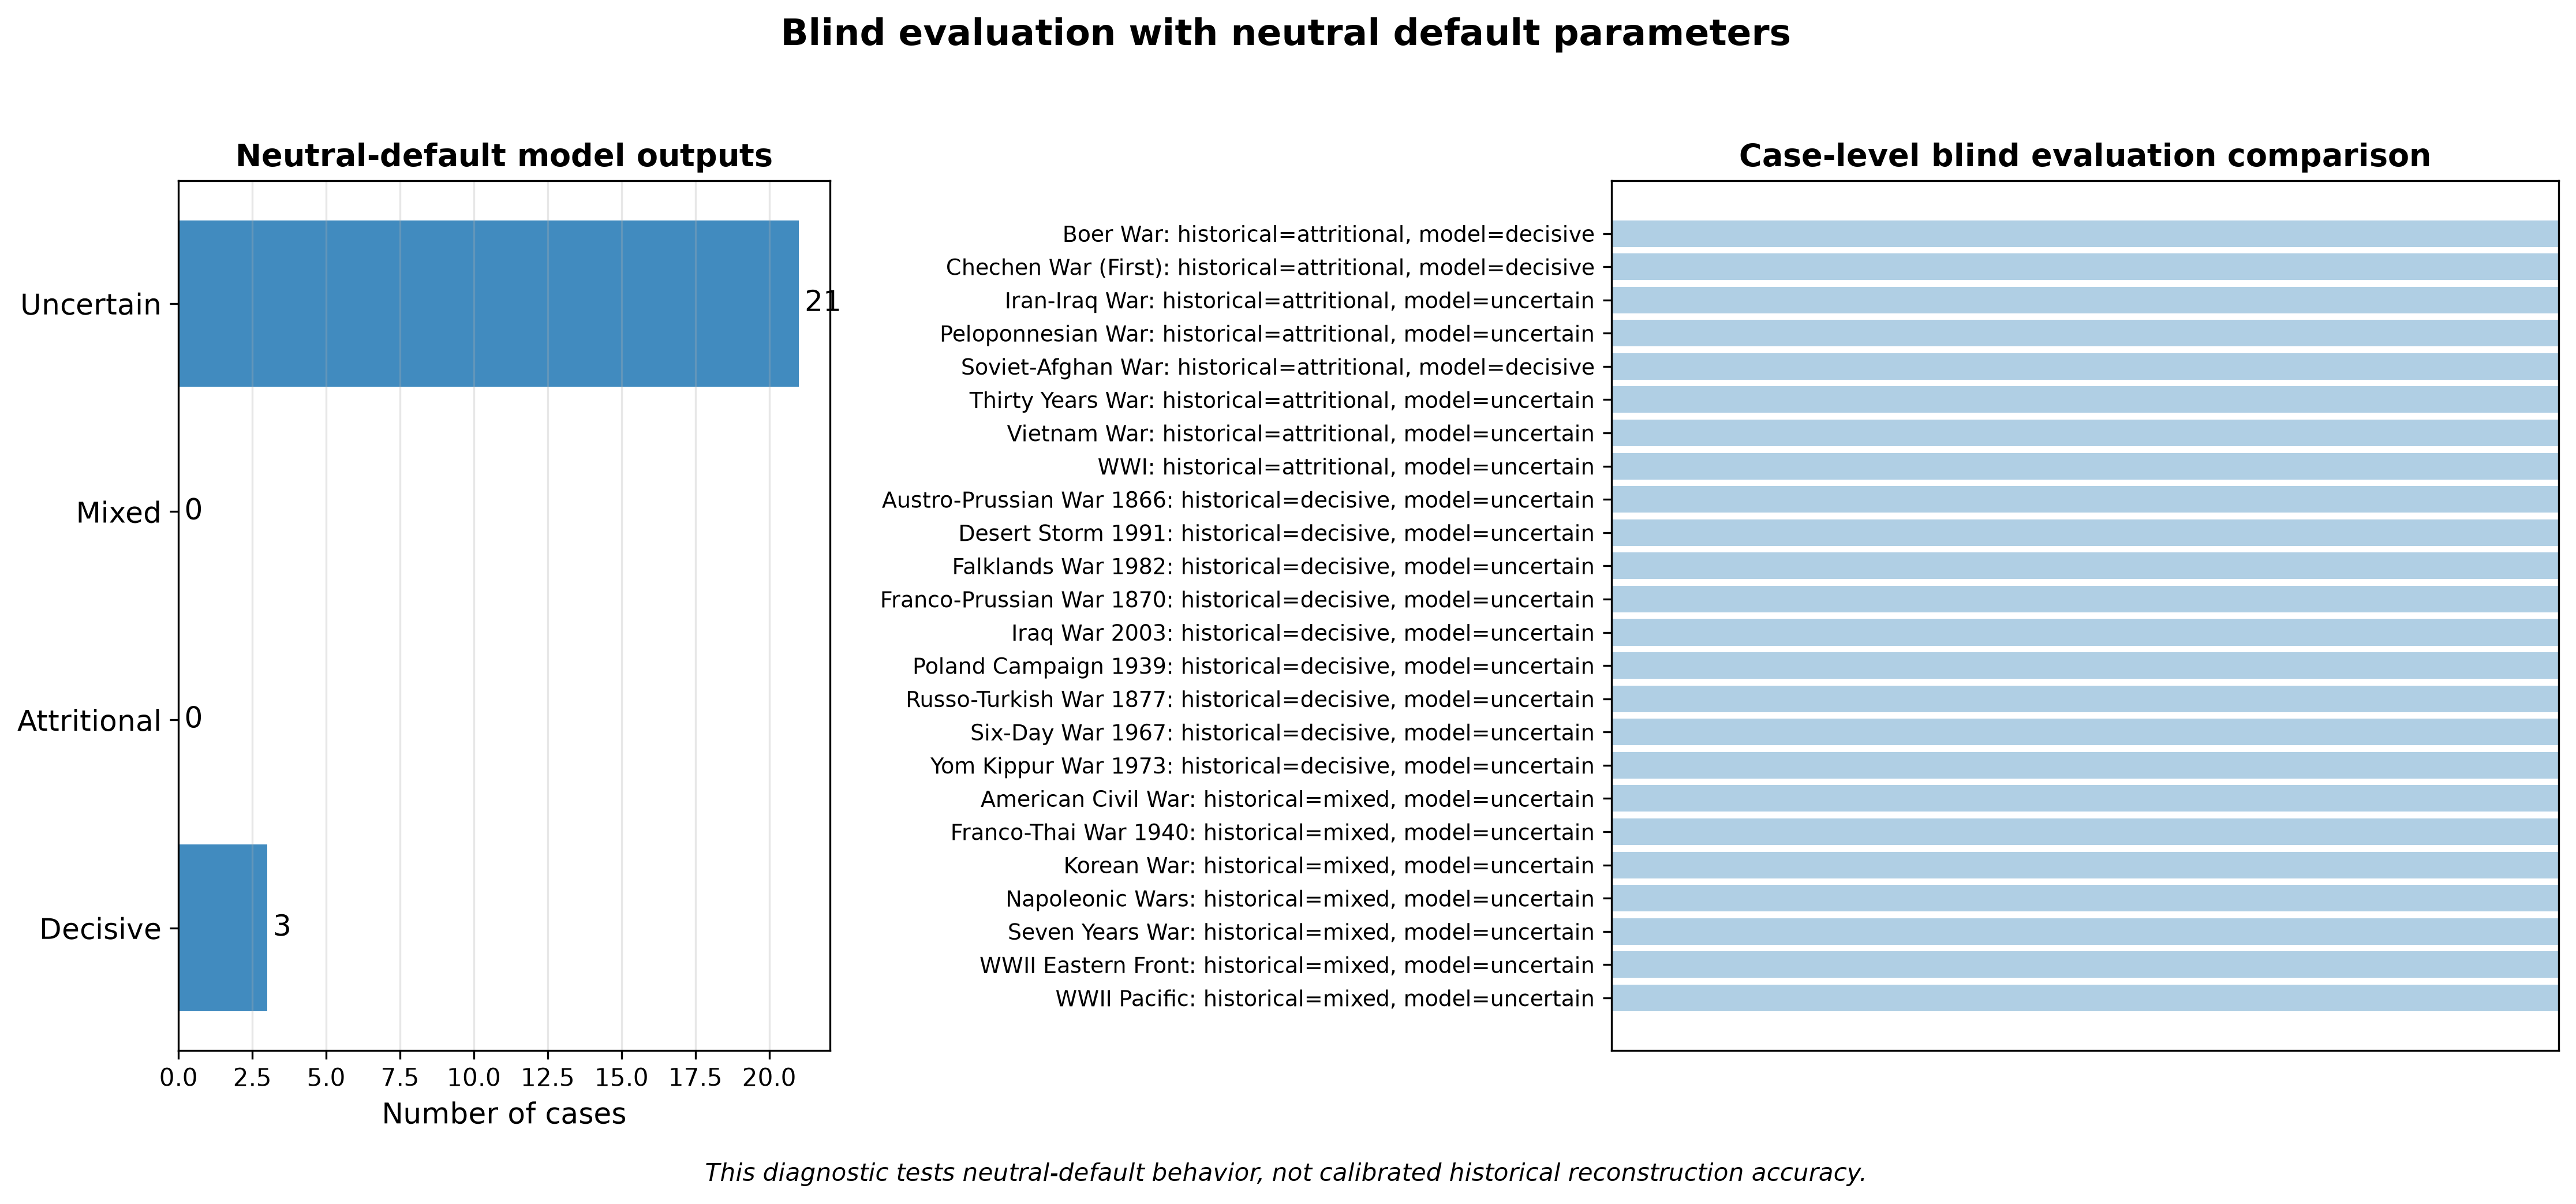
\includegraphics[width=0.8\textwidth]{figures/fig_04_blind_validation.png}
\caption{Blind validation: distribution of preset DSS scores across author-assigned mechanism types (decisive shock, strategic exhaustion, mixed). All cases cluster near the uncertain boundary, confirming that the classifier cannot distinguish mechanisms without case-specific calibration.}
\label{fig:blind_validation}
\end{figure}

\section{ML Model Validation}
\label{app:ml_validation}

The random forest and logistic regression models were validated using 5-fold stratified cross-validation with the following configuration:
\begin{itemize}
    \item Random seed: 42
    \item Cross-validation: Stratified 5-fold
    \item Random forest: 100 trees, max depth 5
    \item Logistic regression: L2 regularization, $C=1.0$, max iterations 2000
    \item Feature scaling: StandardScaler (zero mean, unit variance)
    \item Target: Binary (short war $<$365 days vs.\ long war $\geq$365 days)
    \item Dataset: 2,137 wars with COW National Material Capabilities data
    \item Class balance: 47.7\% short, 52.3\% long
\end{itemize}

The logistic regression achieves 55.0\% $\pm$ 2.2\% cross-validated accuracy (2.7pp above the 52.3\% null baseline), indicating that linear relationships among material-capability features contain limited predictive information. The random forest achieves 72.7\% $\pm$ 1.7\% (AUC = 0.814), indicating that nonlinear interactions among these features contribute substantially to prediction. This 17.7-point gap quantifies the information contained in feature interactions that linear models cannot represent.

\section{Missing Data Severity}
\label{app:missing_data}

Table~\ref{tab:missing_data} quantifies missing data across the seven data sources used in this study. Missing values are imputed to 0 (minimum index contribution), which biases toward uncertainty rather than mechanism classification.

\begin{table}[H]
\centering
\caption{Missing data severity by source and variable. Imputation to 0 reduces index values for incomplete cases.}
\label{tab:missing_data}
\small
\setlength{\tabcolsep}{3pt}
\begin{tabularx}{\textwidth}{@{}>{\RaggedRight\arraybackslash}p{0.22\textwidth} c c >{\RaggedRight\arraybackslash}X@{}}
\toprule
\textbf{Source / Variable} & \textbf{Missing (\%)} & \textbf{Impact} & \textbf{Mitigation} \\
\midrule
\multicolumn{4}{l}{\textit{DSS Components (IWB + Manual)}} \\
\midrule
Casualty concentration & 12\% & High & Imputed to 0; reduces DSS for wars with incomplete battle records \\
Capital capture & 5\% & Low & Binary; missing = no capture \\
Field army destroyed & 8\% & Medium & Binary; missing = not recorded \\
Fleet destroyed & 15\% & Low & Binary; missing = no fleet engagement \\
Rapid surrender & 3\% & Low & Binary; missing = no rapid surrender \\
Regime collapse & 10\% & Medium & Binary; missing = not observed \\
\midrule
\multicolumn{4}{l}{\textit{SES Components (COW + UCDP)}} \\
\midrule
Military expenditure & 22\% & High & Imputed to 0; reduces SES for pre-1949 wars \\
Energy consumption & 35\% & High & Imputed to 0; major gap for pre-SIPRI conflicts \\
Iron \& steel production & 30\% & Medium & Imputed to 0; less critical than energy \\
Battle deaths (annual) & 18\% & Medium & Imputed to 0; reduces cumulative mortality estimate \\
Personnel counts & 15\% & Medium & Imputed to 0; affects manpower depletion metric \\
\midrule
\multicolumn{4}{l}{\textit{Structural DSS Proxy Components}} \\
\midrule
Logistics vulnerability & 100\% & High & Fixed at 50.0; no variation across cases \\
Surprise indicator & 100\% & High & Fixed at 50.0; no variation across cases \\
Alliance asymmetry & 100\% & High & Fixed at 50.0; no variation across cases \\
Mobilization speed & 100\% & High & Fixed at 64.0; no variation across cases \\
Regime stability & 100\% & High & Fixed at 50.0; no variation across cases \\
\bottomrule
\end{tabularx}
\end{table}

\section{Noise Sensitivity}
\label{app:noise_sensitivity}

Table~\ref{tab:noise_sensitivity} reports the results of a Monte Carlo sensitivity analysis with 500 independent noise seeds per historical preset. The noise model adds $\mathcal{N}(0, 0.5)$ to all state variables after each deterministic update step.

\begin{table}[H]
\centering
\caption{Noise sensitivity across 500 seeds per historical preset. Dominant share is the fraction of runs producing the most common termination outcome.}
\label{tab:noise_sensitivity}
\small
\begin{tabularx}{\textwidth}{@{}>{\RaggedRight\arraybackslash}X l c c c c c@{}}
\toprule
\textbf{Case} & \textbf{Dominant outcome} & \textbf{Share} & \textbf{Min} & \textbf{Median} & \textbf{Max} & \textbf{Outcomes} \\
\midrule
Gulf War 1991 & dominance\_a & 1.00 & 13 & 18 & 24 & 1 \\
Vietnam War & withdrawal\_a & 0.79 & 63 & 90 & 124 & 2 \\
Wwi & exhaustion\_b & 0.62 & 54 & 65 & 76 & 2 \\
Franco Prussian & dominance\_a & 1.00 & 9 & 12 & 18 & 1 \\
Korean War & negotiated\_settlement & 1.00 & 40 & 44 & 49 & 1 \\
Iran Iraq & mutual\_exhaustion & 0.97 & 69 & 83 & 102 & 2 \\
Wwii & mutual\_exhaustion & 0.77 & 58 & 68 & 78 & 2 \\
\bottomrule
\end{tabularx}
\end{table}


Three cases show non-trivial noise sensitivity: World War I (62\% dominant share), World War II (77\% dominant share), and the Vietnam War (79\% dominant share). These cases produce two distinct termination outcomes across 500 runs, indicating that the classification boundary is sensitive to stochastic perturbation. The remaining four cases (Gulf War, Franco-Prussian War, Korean War, Iran--Iraq) are highly stable with dominant shares of 97--100\%. The noise-sensitive cases should be interpreted with appropriate caution: their mechanism classifications are probabilistic rather than deterministic.

\section{Statistical Model Audit}
\label{app:statistical_audit}

Table~\ref{tab:statistical_audit} reports the full statistical model audit including variance inflation factors, out-of-bag error, interaction logistic regression, and bootstrap confidence intervals.

\begin{table}[H]
\centering
\caption{Statistical model audit: VIF, out-of-bag error, interaction logistic regression, and bootstrap AUC confidence intervals.}
\label{tab:statistical_audit}
\small
\setlength{\tabcolsep}{4pt}
\begin{tabularx}{\textwidth}{@{}l X r@{}}
\toprule
\textbf{Metric} & \textbf{Details} & \textbf{Value} \\
\midrule
\multicolumn{3}{l}{\textit{Variance Inflation Factors}} \\
energy consumption initial & High & 36.05 \\
cinc pct change & High & 21.79 \\
iron steel initial & High & 18.48 \\
military personnel pct change & High & 16.40 \\
military expenditure initial & Warning & 8.14 \\
military expenditure pct change & OK & 4.56 \\
energy consumption pct change & OK & 4.28 \\
iron steel pct change & OK & 4.11 \\
cinc initial & OK & 3.08 \\
battle deaths initial & OK & 2.49 \\
military personnel initial & OK & 2.18 \\
battle deaths pct change & OK & 1.05 \\
\midrule
\multicolumn{2}{l}{\textbf{Max VIF}} & 36.05 \\
\midrule
\multicolumn{3}{l}{\textit{Model Performance}} \\
Logistic regression test accuracy & 5-fold CV, $C=1.0$ & 0.5483 \\
Logistic regression AUC-ROC & Bootstrap 95\% CI & 0.5610 \\
  LR AUC 95\% CI & $[0.5165,\; 0.6048]$ & \\
Interaction logistic test accuracy & Degree-2 interactions, L2 & 0.5935 \\
Interaction logistic AUC-ROC & & 0.6293 \\
Random forest test accuracy & 100 trees, depth 5 & 0.7321 \\
Random forest AUC-ROC & Bootstrap 95\% CI & 0.7946 \\
  RF AUC 95\% CI & $[0.7598,\; 0.8282]$ & \\
Random forest OOB accuracy & Out-of-bag estimate & 0.7358 \\
\bottomrule
\end{tabularx}
\end{table}


The maximum VIF of 36.05 (energy consumption initial) indicates substantial multicollinearity among the initial-condition features. This is expected: countries with high energy consumption also tend to have high CINC scores, military expenditure, and iron/steel production. The random forest is robust to multicollinearity, but the logistic regression coefficients should be interpreted with caution. The interaction logistic regression (AUC 0.63) provides modest improvement over the baseline logistic (AUC 0.56), while the random forest (AUC 0.79) captures substantially more nonlinear structure. The 95\% bootstrap confidence intervals confirm that the random forest's AUC advantage over logistic regression is statistically significant (non-overlapping intervals).

\section{Empirical vs.\ Simulation Traceability}
\label{app:traceability}

Table~\ref{tab:traceability} maps each claim in the main text to its source: empirical (computed from external data), simulation (computed from model trajectories), or mixed (empirical data fed into simulation). This traceability prevents the conflation of data-derived findings with simulation-generated outputs.

\begin{table}[H]
\centering
\caption{Empirical vs.\ simulation traceability. Each major finding is traced to its data source.}
\label{tab:traceability}
\small
\setlength{\tabcolsep}{3pt}
\begin{tabularx}{\textwidth}{@{}>{\RaggedRight\arraybackslash}p{0.32\textwidth} >{\centering\arraybackslash}p{0.14\textwidth} >{\RaggedRight\arraybackslash}X@{}}
\toprule
\textbf{Finding} & \textbf{Source} & \textbf{Details} \\
\midrule
4,812 wars total & Empirical & Merged COW + Brecke + UCDP datasets \\
91 wars with battle data & Empirical & Interstate War Battle Dataset subset \\
2.2\% decisive shock & Empirical & DSS computed from IWB battle-level data \\
22.0\% strategic exhaustion & Empirical & SES computed from war-year COW data \\
75.8\% uncertain & Empirical & DSS--SES difference $<$ 20 in both directions \\
6/7 mechanism agreement & Mixed & Simulation trajectories compared to author-assigned labels \\
72.7\% RF accuracy & Empirical & Trained on COW NMC features only \\
55.0\% LR accuracy & Empirical & Same features, linear baseline \\
Parameter sensitivity (0.3\% flip) & Simulation & 23 internal coefficients varied $\pm 50\%$ \\
Threshold sensitivity (86.1\% mean) & Simulation & 175 parameter combinations \\
Gulf War = decisive & Mixed & Simulation trajectory consistent with author-assigned label \\
Vietnam = exhaustion & Mixed & Simulation trajectory consistent with author-assigned label \\
Attritional iceberg pattern & Empirical & Distribution of DSS/SES across 91 wars \\
\bottomrule
\end{tabularx}
\end{table}
